\documentclass[a4paper, 10pt]{article}
\usepackage{myresume}  % Style package
\usepackage{hyperref}
\usepackage{graphicx}
\usepackage{geometry}
% remove page number 
\pagenumbering{gobble}
\geometry{left=2cm, right=2cm, top=1.5cm, bottom=1.5cm}
% --------------------  START  --------------------
\begin{document}

% -------------------- HEADING --------------------
\begin{flushright}
  % \setstretch{0.6}
  % \item {\Calluna (+00) 111-2222-3333}  % Phone number
  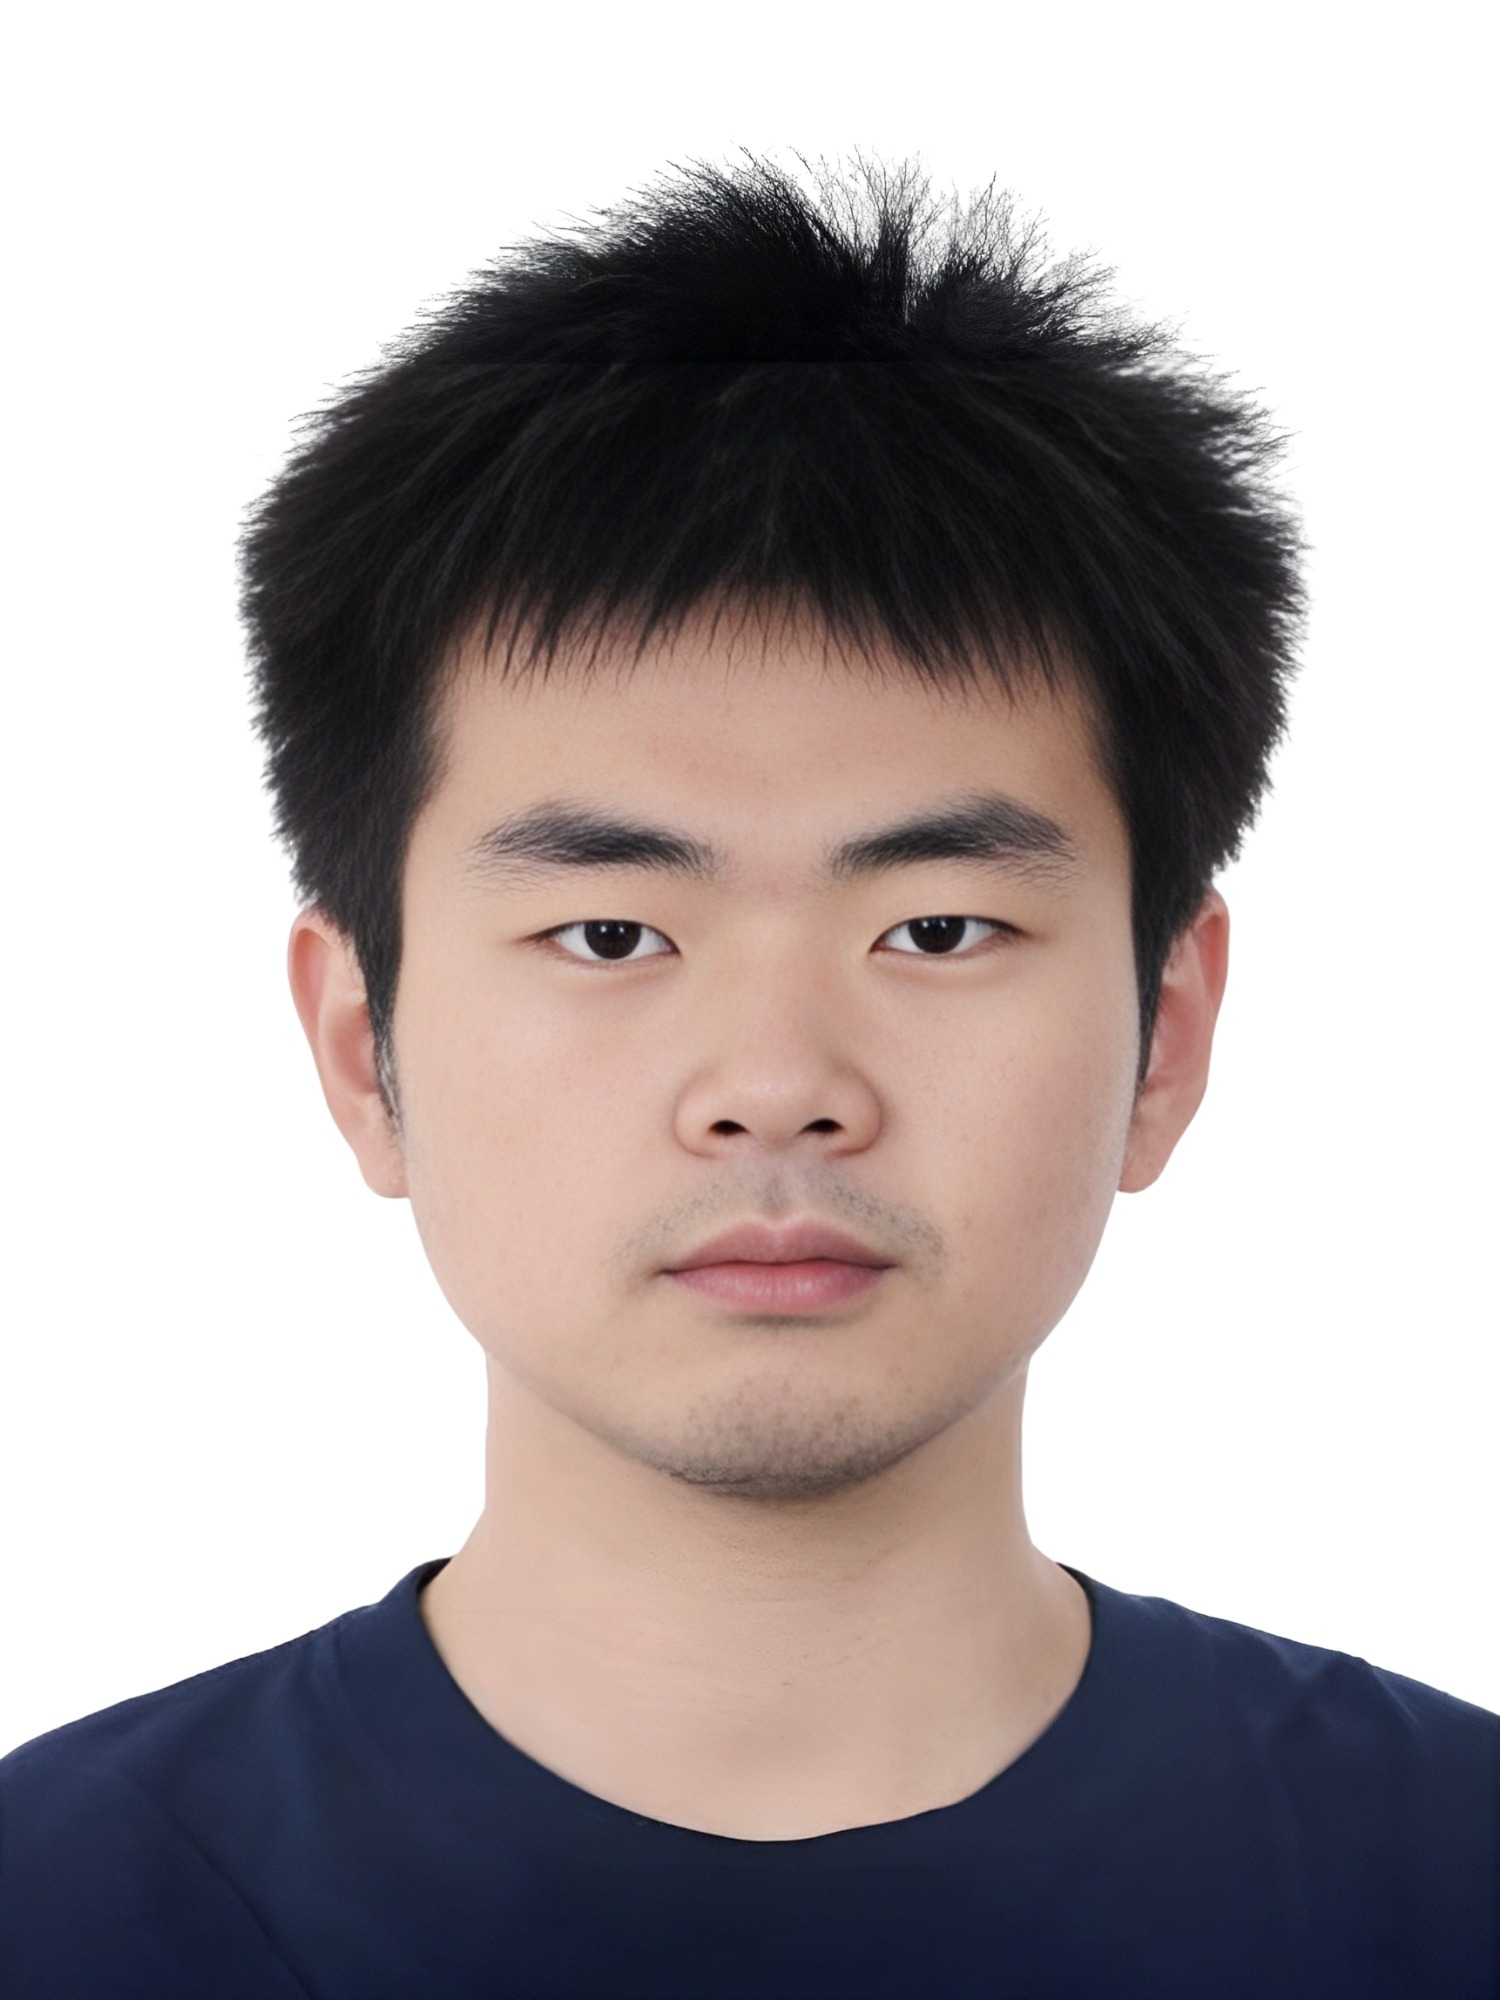
\includegraphics[width=2.5cm]{../assets/img/self-white}
\end{flushright}\vspace{-90pt}

\begin{flushleft}  % Rplace here with your name (and identity if required)
  {\Calluna \fontsize{30pt}{30pt}\selectfont \textsc{\unskip Yiren Lu} } \quad {\Calluna \fontsize{14.5pt}{14.5pt}}
  \vspace{1em}

  \item {\Calluna luyiren12@gmail.com}  % E-mail address
  \item {\Calluna \url{ https://yiren.lu}}  % Home page
  
  \noindent\rule{0.83\textwidth}{0.4pt}
\end{flushleft}



% -------------------- EDUCATION --------------------
\sectionBlock{
  \section{Education}
}{
  
  \eduHeading
  {\unskip Institute of Computing Technology, Chinese Academy of Sciences}{\unskip Beijing, China}
  {\unskip Master's candidate  in  Computer Software and Theory}{ 2022.08 - present}
  
  \itemListStart
  
  \myItem{\unskip Advisor: Xiaoming Sun}
  
  \myItem{\unskip Research area: quantum computation, theoretical computer science}
  
  \itemListEnd
  
  
  \eduHeading
  {\unskip School of Computer Science, Beijing University of Posts and
Telecommunications}{\unskip Beijing, China}
  {\unskip Bachelor of Engineering  in  Computer Science and Technology}{ 2018.09 - 2022.07}
  
  \itemListStart
  
  \myItem{\unskip GPA: 90.34/100 (5\%)}
  
  \itemListEnd
}


% -------------------- PUBLICATIONS --------------------
\sectionBlock{
  \section{Research}
}{
  \pubListStart
  \justifying
  
  \item \textbf{Yiren Lu}, Junhong Nie, Xiaoming Sun, Guojing Tian. Optimized synthesis of 2-degree parity network.\textit{ In submission}, 2024.
  
  \item \textbf{Yiren Lu}, Guojing Tian, Xiaoming Sun. QAOA with fewer qubits: a coupling framework to solve larger-scale
Max-Cut problem.\textit{ arXiv preprint arXiv:2307.15260}, 2023.
  
  \pubListEnd
}

% -------------------- AWARDS & HONORS --------------------
\sectionBlock{
  \section{Awards\\and\\Honors}
}{
  \awardListStart
  \justifying
  
  \item \emph{\unskip CCF Outstanding Undergraduate Award},{ China Computer Federation} \hfill 2021.08
  
  \item \emph{\unskip Gold Medal (ranking 6/1000+)},{ CCF Collegiate Computer Systems \& Programming Contest (CCSP 2020)} \hfill 2020.10
  
  \item \emph{\unskip Silver Medal},{ International Collegiate Programming Contest (ICPC), Asia East Continent
Final} \hfill 2019.12
  
  \item \emph{\unskip Silver Medal},{ China Collegiate Programming Contest (CCPC), Guilin Onsite} \hfill 2018.11
  
  \item \emph{\unskip Bronze Medal},{ National Olympiad in Informatics (NOI 2017)} \hfill 2017.07
  
  \item \emph{\unskip Silver Medal},{ National Olympiad of Informatics' Winter Camp (WC 2017)} \hfill 2017.02
  
  \awardListEnd
}


\sectionBlock{
  \section{Interests}
}{
  \skillListStart
  \justifying
  
  \item \emph{\unskip Quantum computation}: {  }quantum circuit synthesis, variational quantum algorithms
  \item \emph{\unskip Graph theory}: {  }recognition of graph classes, quantum speed-up for graph problems
  \item \emph{\unskip Other random topics}: {  }approximation algorithms, computational complexity
  \skillListEnd
}


\sectionBlock{
  \section{Teaching Assistants}
}{
  \skillListStart
  \justifying
  
  \item \emph{\unskip Quantum Computation and Quantum Software}
  
  University of Chinese Academy of Sciences\hfill Spring 2024
  
  \item \emph{\unskip Data Structures I}
  
  Renmin University of China\hfill Autumn 2024
  
  \skillListEnd
}



% -------------------- SKILLS --------------------
\sectionBlock{
\section{Skills}
}{
\skillListStart
\justifying
\item \emph{Languages}: Chinese, English (TOEFL 106, GRE 324+4)
\item \emph{Programming}: \texttt{Python}, \texttt{C++}, \texttt{JavaScript}, \texttt{LaTeX}
\item \emph{Cooking}
\skillListEnd
}

% -------------------- OTHERS --------------------
\sectionBlock{
  \section{Academic Services}
}{
  \skillListStart
  \justifying
  
  \item \emph{\unskip Reviewer}:\textit{ Quantum Science and Technology}
  \skillListEnd
}

\end{document}

